\documentclass[12pt]{article}
 
\usepackage[margin=1in]{geometry} 
\usepackage{amsmath,amsthm,amssymb}
\usepackage{graphicx}
\usepackage{tikz}
\usepackage{tikz-qtree}
\usepackage{wrapfig}
\usepackage{marvosym}
\usetikzlibrary{calc,patterns,angles,quotes}
 
\newcommand{\N}{\mathbb{N}}
\newcommand{\Z}{\mathbb{Z}}
\newcommand{\R}{\mathbb{R}}
\newcommand{\C}{\mathbb{C}}

\usepackage{mathtools}

%\DeclarePairedDelimiter\ceil{\left\lceil}  {\right\rceil}
%\DeclarePairedDelimiter\floor{\left\lfloor}{\right\rfloor}
 
\usepackage{amsthm}
\newtheorem{proposition}{Proposition}
\newtheorem{question}{Question}                                                                                                                                                                                          
 
\begin{document}
 
\title{Solutions to Exercise Sheet 6}
\author{Leif Van Holland \\ \\
\textsc{Discrete and Computational Geometry}}

\maketitle

\section*{Exercise 16}
Given the set $S=\{0,4,5,7,12,13,14,16\}$, we get the following split-tree $T$:
\begin{figure}[h]
    \centering
    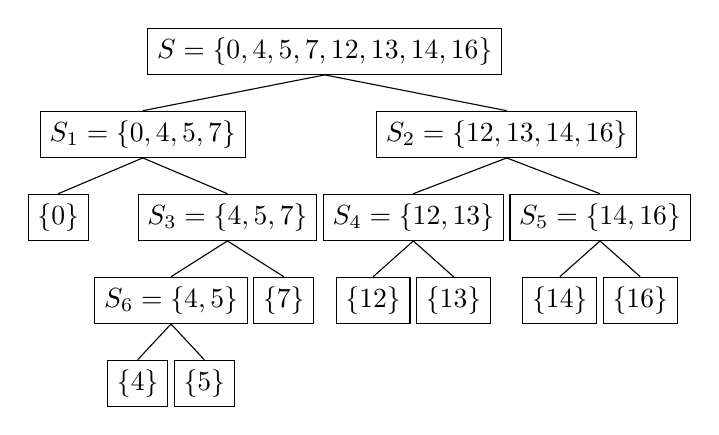
\begin{tikzpicture}[%
        every node/.style={rectangle, draw=black},
        level 1/.style={level distance=3em},
        level 2/.style={level distance=3em},
        level 3/.style={level distance=3em},
        level 4/.style={level distance=3em}
        ]
        \Tree [.$S=\{0,4,5,7,12,13,14,16\}$
                [.$S_1=\{0,4,5,7\}$
                    [.$\{0\}$ ]
                    [.$S_3=\{4,5,7\}$
                        [.$S_6=\{4,5\}$
                            [.$\{4\}$ ]
                            [.$\{5\}$ ]
                        ]
                        [.$\{7\}$ ]
                    ]
                ]
                [.$S_2=\{12,13,14,16\}$
                    [.$S_4=\{12,13\}$
                        [.$\{12\}$ ]
                        [.$\{13\}$ ]
                    ]
                    [.$S_5=\{14,16\}$
                        [.$\{14\}$ ]
                        [.$\{16\}$ ]
                    ]
                ]
              ]
    \end{tikzpicture}
\end{figure}
To construct the WSPD of $T$ for $s=3$, we have to run \texttt{FindPairs} for the children $v_1,v_2$ of every inner node. The procedure checks if the distance of the centers $c_1, c_2$ of the smallest enclosing circle of all points in the corresponding sets of the children is greater than $(s+2)\cdot r = 5r$, where $r$ denotes the radius of the bigger enclosing circle. If the distance is smaller, \texttt{FindPairs} will be called recursively, splitting the bigger set in accordance to $T$.\par
\noindent This results in the following calls to \texttt{FindPairs}:
\begin{itemize}
    \item FP($S_1, S_2$): $c_1=3.5, c_2=14, r=3.5\quad$ and $\quad|c_1c_2| = 11.5 < 5\cdot r = 17.5 \:$
    \Lightning
    \begin{itemize}
        \item FP($\{0\}, S_2$): $c_1=0, c_2=14, r=2\quad$ and $\quad|c_1c_2| = 14 > 5\cdot r = 10 \:$ \checkmark
        \item FP($S_3, S_2$): $c_1=5.5, c_2=14, r=2\quad$ and $\quad|c_1c_2| = 9.5 < 5\cdot r = 10 \:$ \Lightning
        \begin{itemize}
            \item FP($S_3, S_4$): $c_1=5.5, c_2=12.5, r=1.5\quad$ and $\quad|c_1c_2| = 7 < 5\cdot r = 7.5 \:$ \Lightning
            \begin{itemize}
                \item FP($S_6, S_4$): $c_1=4.5, c_2=12.5, r=0.5\:$ and $\:|c_1c_2| = 8 > 5\cdot r = 2.5 \:$ \checkmark
                \item FP($\{7\}, S_4$): $c_1=7, c_2=12.5, r=0.5\:$ and $\:|c_1c_2| = 7.5 > 5\cdot r = 2.5 \:$ \checkmark
            \end{itemize}
            \item FP($S_3, S_5$): $c_1=5.5, c_2=15, r=2\quad$ and $\quad|c_1c_2| = 9.5 > 5\cdot r = 7.5 \:$ \checkmark
        \end{itemize}
    \end{itemize}
        
    \item FP($\{0\}, S_3$): $c_1=0, c_2=5.5, r=1.5\quad$ and $\quad|c_1c_2| = 5.5 < 5\cdot r = 7.5 \:$ \Lightning
    \begin{itemize}
        \item FP($\{0\}, S_6$): $c_1=0, c_2=4.5, r=0.5\:$ and $\:|c_1c_2| = 4.5 > 5\cdot r = 2.5 \:$ \checkmark
        \item FP($\{0\}, \{7\}$): $r=0\:$ \checkmark
    \end{itemize}
    
    \item FP($S_4, S_5$): $c_1=12.5, c_2=15, r=1\quad$ and $\quad|c_1c_2| = 2.5 < 5\cdot r = 5 \:$ \Lightning
    \begin{itemize}
        \item FP($S_4, \{14\}$): $c_1=12.5, c_2=14, r=0.5\quad$ and $\quad|c_1c_2| = 1.5 < 5\cdot r = 2.5 \:$ \Lightning
        \begin{itemize}
            \item FP($\{12\}, \{14\}$): $r=0\:$ \checkmark
            \item FP($\{13\}, \{14\}$): $r=0\:$ \checkmark
        \end{itemize}
        \item FP($S_4, \{16\}$): $c_1=12.5, c_2=16, r=0.5\:$ and $\:|c_1c_2| = 3.5 > 5\cdot r = 2.5 \:$ \checkmark
    \end{itemize}
    
    \item FP($S_6, \{7\}$): $c_1=5.5, c_2=7, r=0.5\:$ and $\:|c_1c_2| = 1.5 < 5\cdot r = 2.5 \:$ \Lightning
    \begin{itemize}
        \item FP($\{4\}, \{7\}$): $r=0\:$ \checkmark
        \item FP($\{5\}, \{7\}$): $r=0\:$ \checkmark
    \end{itemize}
    
    \item FP($\{12\}, \{13\}$): $r=0\:$ \checkmark
    \item FP($\{14\}, \{16\}$): $r=0\:$ \checkmark
    \item FP($\{4\}, \{5\}$): $r=0\:$ \checkmark
    
\end{itemize}

The resulting WSPD therefore contains the following pairs:
\[ (\{0\}, S_2), (S_6,S_4), (\{7\}, S_4), (S_3,S_5), (\{0\}, S_6), (\{0\},\{7\}), (\{12\},\{13\}), \]
\[ (\{13\},\{14\}), (S_4, \{16\}), (\{4\},\{7\}), (\{5\},\{7\}), (\{12\},\{13\}),  (\{14\},\{16\}), (\{4\},\{5\}). \]
To calculate the $k=3$ nearest neighbors, we first have to construct the candidate lists $L(a)$ for every point $a\in S$. To get these lists, we require candidate lists $N(B)$ for the sets $B$ of all nodes in $T$. These lists are initialized as
\[N(B)_{\text{init}}=N(\text{parent}(B)) \cup I(B),\: I(B):=\{a\: |\: \exists A, a\in A, |A|\leq k, (A,B)\in\text{WSPD}\}.\]
and then we construct a $\frac{1}{2}$-frame and assign all points in $N(B)_\text{init}$ to the cones of the $\frac{1}{2}$-frame. Because the points are from $\R$, the $\frac{1}{2}$-frame consists of the intervals $[o_B,\infty)$ and $(-\infty,o_B]$, where $o_B$ denotes the center of $B$. For each interval we calculate the distance of all assigned points to $o_B$ and remove all points from $N(B)_\text{init}$ that are farther away than the $k$-th closest point assigned to the interval.\par

Before we determine the initial lists, we compute $I(B)$ for every node:
\begin{align*}
  I(S_1) &= \varnothing, \quad &I(S_2) &= \{0\}, \quad &I(\{0\}) &= \{4,5,7\}, \\  
  I(S_3) &= \{14,16\}, \quad &I(S_4) &= \{4,5,7,16\},\quad &I(S_5) &= \{4,5,7\},  \\
  I(S_6) &= \{0,12,13\}, \quad &I(\{7\}) &= \{0,4,5,12,13\}, \quad &I(\{12\}) &= \{13,14\}, \\
  I(\{13\}) &= \{12,14\}, \quad &I(\{14\}) &= \{12,13,16\}, \quad &I(\{16\}) &= \{12,13,14\},\\
  \quad I(\{4\}) &= \{5,7\}, \quad &I(\{5\}) &= \{4,7\}.
\end{align*}

Using the method described above, we get the following $N(B)_\text{init}$ and $N(B)$:
\begin{align*}
    N(S) &:= \varnothing \\
    N(S_1)_\text{init} &= \varnothing \cup \varnothing = \varnothing = N(S_1) \\
    N(S_2)_\text{init} &= \varnothing \cup \{0\} = N(S_2) \\
    N(\{0\})_\text{init} &= \varnothing \cup \{4,5,7\} = N(\{0\}) \\
    N(S_3)_\text{init} &= \varnothing \cup \{14,16\} = N(S_3) \\
    N(S_4)_\text{init} &= \{0\} \cup \{4,5,7,16\} \\
    o_{S_4} &= 8 \implies N(S_4) = \{4,5,7\} \cup \{16\} \\
    N(S_5)_\text{init} &= \{0\} \cup \{4,5,7\} \\
    o_{S_5} &= 3.5 \implies N(S_5) = \{0\} \cup \{4,5,7\} \\
    N(S_6)_\text{init} &= \{14,16\} \cup \{0,12,13\} \\
    o_{S_5} &= 8 \implies N(S_6) = \{0\} \cup \{12,13,14\} \\
    N(\{7\})_\text{init} &= \{14,16\} \cup \{0,4,5,12,13\} \\
    o_{\{7\}} &= 6.5 \implies N(\{7\}) = \{0,4,5\} \cup \{12,13\} \\
    N(\{12\})_\text{init} &= \{4,5,7,16\} \cup \{13,14\} \\
    o_{\{12\}} &= 8 \implies N(\{12\}) = \{4,5,7\} \cup \{13,14,16\} \\
    N(\{13\})_\text{init} &= \{4,5,7,16\} \cup \{12,14\} \\
    o_{\{13\}} &= 8 \implies N(\{13\}) = \{4,5,7\} \cup \{12,14,16\} \\
    N(\{14\})_\text{init} &= \{0,4,5,7\} \cup \{12,13,16\} \\
    o_{\{14\}} &= 8 \implies N(\{14\}) = \{4,5,7\} \cup \{12,13,16\} \\
    N(\{16\})_\text{init} &= \{0,4,5,7\} \cup \{12,13,14\} \\
    o_{\{16\}} &= 7 \implies N(\{16\}) = \{4,5,7\} \cup \{12,13,14\} \\
    N(\{4\})_\text{init} &= \{0,12,13,14\} \cup \{5,7\} \\
    o_{\{4\}} &= 7 \implies N(\{4\}) = \{0,5,7\} \cup \{12,13,14\} \\
    N(\{5\})_\text{init} &= \{0,12,13,14\} \cup \{4,7\} \\
    o_{\{5\}} &= 7 \implies N(\{5\}) = \{0,4,7\} \cup \{12,13,14\}
\end{align*}
To retrieve the lists $L(a)$, we iterate over all $N(\{b\})$ and assigning a point $b$ to $L(a)$, if $a\in N(\{b\})$. This yields:
\begin{align*}
    L(0) &= \{7,4,5\}, \quad &L(4) &= \{0,7,12,13,14,16,5\}, \\
    L(5) &= \{0,7,12,13,14,16,4\}, \quad &L(7) &= \{0,12,13,14,16,4,5\}, \\
    L(12) &= \{7,13,14,16,4,5\}, \quad &L(13) &= \{7,12,14,16,4,5\}, \\
    L(14) &= \{12,13,16,4,5\}, \quad &L(16) &= \{12,13,14\}.
\end{align*}
Again, removing all points that are farther away from $a$ than the $k$-th closest in every $L(a)$, we get the $k$-nearest neighbors of every $a$:
\begin{align*}
    3\text{NN}(0) &= \{4,5,7\}, \quad &3\text{NN}(5) &= \{0,5,7\}, \quad &3\text{NN}(5) &= \{0,4,7\}, \\
    3\text{NN}(7) &= \{4,5,12\}, \quad &3\text{NN}(12) &= \{7,13,14\}, \quad &3\text{NN}(13) &= \{12,14,16\}, \\
    3\text{NN}(14) &= \{12,13,16\}, \quad &3\text{NN}(16) &= \{12,13,14\}.
\end{align*}

\section*{Exercise 17}
Let $A\subset \R^d$ be a set containing a single point and $B\subset \R^d$ be the unit-hypercube.
\begin{itemize}
    \item [a)] For a $d$-dimensional volume, we know that $\text{vol}(t\cdot B) = t^d\: \text{vol}(B)$. Also, a set consisting only one point has a volume of $0$. Therefore we get
    \[ v(t) = \text{vol}(\underbrace{(1-t)\cdot A}_{=0} +\: t\cdot B) = \text{vol}(t\cdot B) = t^d\cdot \underbrace{\text{vol}(B)}_{=1} = t^d.  \]
    \item [b)] \textbf{Proposition.} \textit{$v(t)^\beta$ is not concave on $[0,1]$ for any $\beta > \frac{1}{d}$.}
    \begin{proof}
    Assume that $v(t)^\beta$ is concave on $[0,1]$ with $\beta > \frac{1}{d}$. This is equivalent to
    \[ \forall a,b,t\in[0,1] \text{ with } a \leq t \leq b:\: v(t)^\beta > v(a)^\beta\left(1-\frac{t-a}{b-a}\right)+v(b)^\beta\:\frac{t-a}{b-a} \]
    To simplify this condition, w.l.o.g. we can assume $a=0,b=1$, as we could scale $v(t)^\beta$ accordingly. This gives
    \[ \forall t\in[0,1]: v(t)^\beta > v(0)^\beta\:(1-t)+v(1)^\beta\: t \]
    From a) we know that
    \[v(t)^\beta=t^{d\cdot \beta}=t^{-k} \text{ for a } k > 1\]
    but this yields
    \[v(0)^\beta\:(1-t) + v(1)^\beta\:t = 0^{-k}\cdot (1-t) + 1^{-k} \cdot t = t \overset{\text{\Lightning}}{\leq} t^{-k} = v(t)\]
    which contradicts the concavity condition. Therefore the assumption that $v(t)^\beta$ is concave must be wrong.
    \end{proof}
    
\end{itemize}

\end{document}